\section*{Avant Propos}

Afin d'analyser et classifier des images 2D ou imageries 3D, il est primordial d'être capable d'extraire de ces dernières un ensemble d'informations ou "\textit{features}" qui décrivent au mieux et nous renseigne sur la nature de celle-ci.\\
On pourrait citer par exemple des critères comme la taille de la boite englobante (en anglais : \textit{bounding box}), ou encore le volume de la forme pour une pièce mécanique en 3D, en passant par la surface de cette dernière. Le critères isopérimétrique (mesure de compacité) est un excellent exemple de facteur classifiant. Il permet de discriminer, avec une bonne précision, différentes pièces mécaniques à partir de modèle 3D [M. Bruneau et al]~\cite{Bruneau2014}.

Dans le cadre de ce stage, nous nous focaliserons sur :\\
\begin{itemize}
	\item	L'accent sera porté sur une analyse d'\textbf{images en 2D}.\\
	\item	Nous cherchons à rétro-concevoir de grands ensembles mécaniques, une attention à la gestion de \textbf{grands volumes de données} doit être apportée durant tout le déroulement du projet.\\
	\item	Mettre en place une \textbf{méthode d'extraction} de descripteurs d'un fichier image (en anglais : \textit{Feature Extractor}).\\
	\item	Cette \textbf{méthode} d'extraction doit être \textbf{automatisable}. Il n'est pas envisageable, dans le cadre de notre étude, de venir renseigner à la main chacun de ces descripteurs.	
\end{itemize}
\vspace{3mm}
  

\section{Les Shock Graphs}

\subsection{État de l'art et méthodes d'extraction de descripteurs.}

Suite à trois semaines d'analyse de la littérature scientifique, il en est ressorti plusieurs méthodes qui pourraient satisfaire nos besoins. La plupart de ces méthodes sont directement dérivées du domaine de la \textbf{Vision par Ordinateur}.

J'ai testé plusieurs méthodes basées sur différentes approches du problèmes :
\begin{itemize}
	\item Filtre de Canny
	\item Algorithme SURF
	\item Réseaux de Convolutions
	\item Shock Graphs
	\item \ldots
\end{itemize}
\vspace{3mm}

\begin{figure}[H]
    \centering
    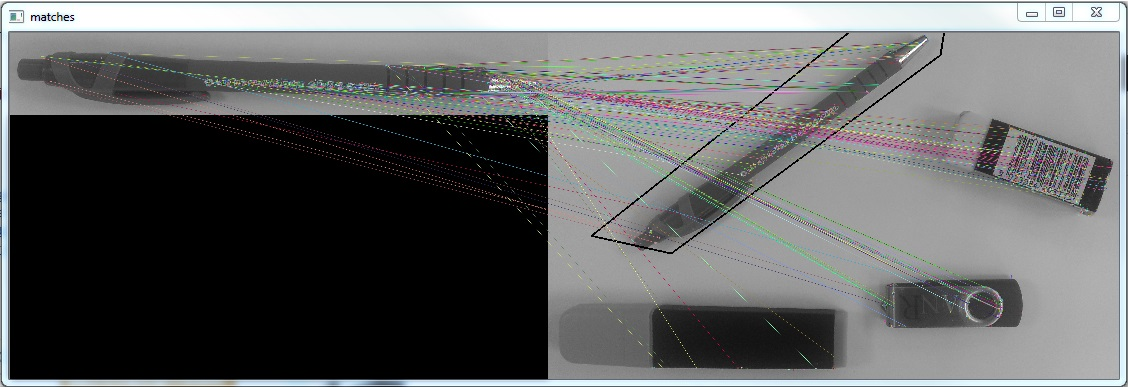
\includegraphics[height=5.5cm]{CannySurfClean.jpg}
	\caption{Output d'un test avec l'algorithme SURF, cible totalement visible} 
\end{figure}
\vspace{-6mm}

\begin{figure}[H]
    \centering
    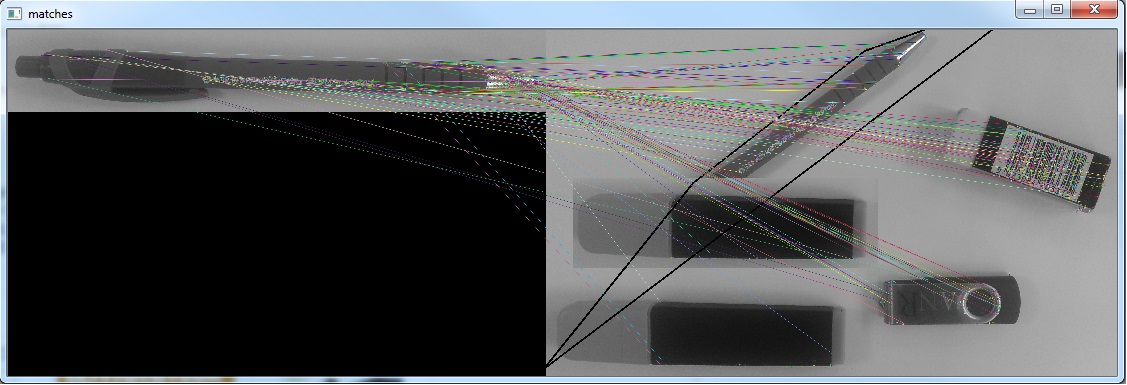
\includegraphics[height=5.5cm]{CannySurfPartiallyMasked.jpg}
	\caption{Output d'un test avec l'algorithme SURF, cible partiellement visible}\label{image.CannySurfPartiallyMasked} 
\end{figure}
\vspace{-6mm}

Il apparait que l'algorithme SURF manque de précision et vient \textit{accrocher} tous les objets de la scène. D'avantages d'investigations ont mis en évidence que l'algorithme étant basé sur la détection de points d'intérêt n'est pas capable d'apprendre une forme mais uniquement les détails d'un objet spécifique. Raisons qui font de l'algorithme SURF un \textbf{mauvais candidat} pour notre étude.

\clearpage
\subsection{Tests préliminaires sur le fonctionnement des Shock Graphs}

Suite à mes recherches bibliographiques, j'ai pu mettre en évidence les travaux sur les Shock Graphs. Ce sont des graphs qui décrivent une forme binaire 2D (Blanche ou Noire, pas de gris) par le biais d'un \textit{squelette} ou \textit{axe médian de Blum}. Leur fonctionnement et leur utilisation est décrite par [K. Siddiqi et al]~\cite{Siddiqi1999}. Un démonstrateur scientifique et une méthode de comparaison de ces graphs a été mise au point par [D. Macrini et al]~\cite{Macrini2002} dans le cadre de son mémoire de master.

À partir de ces travaux, j'ai pu mettre sur pied assez rapidement un test mettant en évidence la pertinence de la méthode relative à notre usage. Et je dois bien admettre avoir été bluffé par la précision de cette méthode. Sentiment qui semble avoir partagé autour de moi.

J'ai créé donc pour le test un jeu de données d'apprentissage et un jeu de test. Chacun contenant un ensemble de vues des pièces mécaniques suivantes:
\begin{itemize}
	\item 	Piston
	\item	Bielle
	\item	Assemblage Piston/Bielle
	\item	Roue dentée
\end{itemize}
\vspace{5mm}

\begin{figure}[H]
    \centering
    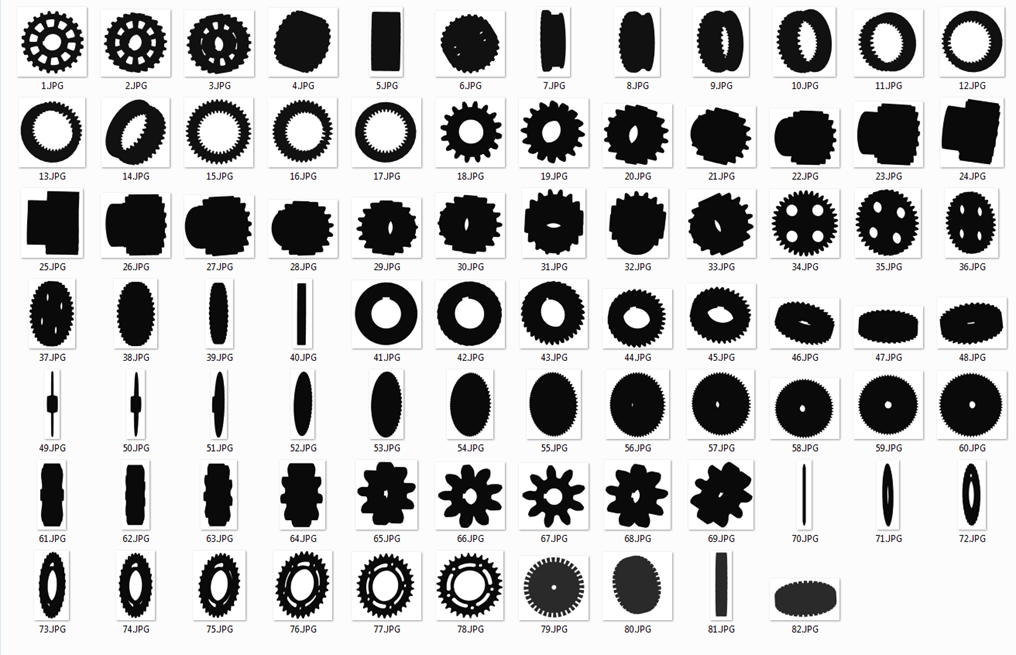
\includegraphics[height=7cm]{datasetShock.png}
	\caption{Exemple de base de connaissances sur les roues dentées, en vue du test des Shock Graphs}\label{image.ShockGearDataset} 
\end{figure}
\vspace{-4mm}

\begin{figure}[H]
    \centering
    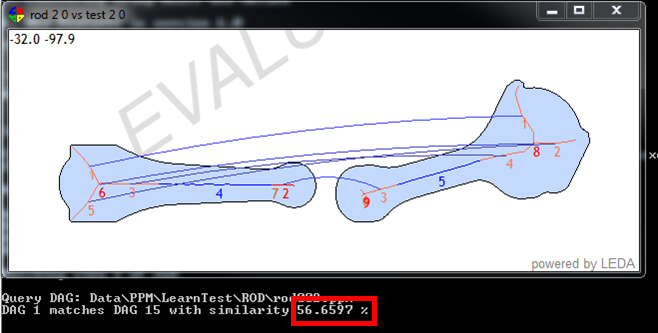
\includegraphics[height=5.5cm]{ShockTest1.png}
	\caption{Output d'un test utilisant les Shock Graphs, \textbf{56.6597\% de match}.}\label{image.ShockTest1} 
\end{figure}


\clearpage

\subsection{Principe de fonctionnement des Shock Graphs.}

Lotus Notes (solution logicielle développée par \textbf{IBM}) et Cordys Process Factory (solution Cloud développée \textbf{Open~Text}) ont un objectif commun : proposer une réponse au  besoin de ``\textit{Business Processing}" au sein d'une entreprise.

Cependant elles diffèrent sur l'architecture (serveurs et réseau) nécessaire à son fonctionnement :

\begin{itemize}
		\item Lotus Notes se base sur une architecture type logiciel Client / logiciel Serveur, les serveurs sont inter-connectés entre eux et ``\textit{répliquent}" certaines de leur données à intervalle de temps régulier. Ce fonctionnement est coûteux , il demande une infrastructure imposante ainsi qu'une administration au jour le jour. \\
		Plus gênant, comme il est difficile d'avoir une vue d'ensemble du système actuel, la quantité d'application dupliquée ne cesse d'augmenter, ce qui induit des coûts de fonctionnement de plus en plus élevés.\\

	\item Cordys Process Factory propose une réponse orientée ``\textit{Cloud Computing}" à ces problématiques, nous pouvons donc faire \textit{abstraction} de l'architecture réseau et serveur nécessaire à son fonctionnement (gérée par le fournisseur du service). La plateforme est accessible via un navigateur web, nul besoin de paramétrer son ordinateur ou d'installer un quelconque logiciel.\\
	Le choix de Cordys Process Factory est donc cohérent avec la politique actuelle du groupe Valeo qui cherche à \emph{externaliser} la gestion de la partie infrastructure et l'administration des diverses solutions informatiques.\\
	\end{itemize}


Valeo a fait le choix de se baser en grande partie sur la suite Google Apps pour un maximum de services et besoins bureautiques. Ainsi nous utilisons de manière non exclusive: 

	\begin{itemize}
		\item Gmail
		\item Google Drive
		\item Google Apps (SpreadSheet, Docs, Presentation, Scripts, Sites)
		\item Google Agenda 
		\item Google AppEngine
	\end{itemize}

En complément nous utilisons un LDAP, commun à tous les sites Valeo du monde, interfacé avec la suite applicative de \textbf{Google}. Valeo appelle cet ensemble de systèmes inter-opérants  : VeGA \textit{(Valeo empowered by Google Apps)}.

\textbf{Et \textit{Cordys Process Factory} dans tout ça ?}

Fort de sa position de partenaire \emph{Google Entreprise}, Cordys Process Factory permet une inter-connection aux services Google Apps  et le LDAP de Valeo : \textit{l'Entreprise Directory}.\\
Ainsi les \textit{Businness Process} et \textit{Businness Workflows} peuvent s'appuyer sur les services et applications déjà en place chez Valeo afin de réduire les coûts de mise en place et de développement.

\clearpage